\documentclass[]{article}
\renewcommand*\sfdefault{uop}
\renewcommand*\familydefault{\sfdefault} %% Only if the base font of the document is to be sans serif
\usepackage[T1]{fontenc}
\usepackage{lmodern}
\usepackage{amssymb,amsmath}
\usepackage{ifxetex,ifluatex}
\usepackage{titlesec}
\titleformat*{\section}{\LARGE\fontfamily{ppl}\selectfont}
\titleformat*{\subsection}{\Large\fontfamily{ppl}\selectfont}
\titleformat*{\subsubsection}{\large\fontfamily{ppl}\selectfont}
\usepackage{fixltx2e} % provides \textsubscript
% use upquote if available, for straight quotes in verbatim environments
\IfFileExists{upquote.sty}{\usepackage{upquote}}{}
\ifnum 0\ifxetex 1\fi\ifluatex 1\fi=0 % if pdftex
  \usepackage[utf8]{inputenc}
\else % if luatex or xelatex
  \usepackage{fontspec}
  \ifxetex
    \usepackage{xltxtra,xunicode}
  \fi
  \defaultfontfeatures{Mapping=tex-text,Scale=MatchLowercase}
  \newcommand{\euro}{€}
    \setmainfont{uop}
    \setsansfont{uop}
    \setmonofont{BeraMono}
\fi
% use microtype if available
\IfFileExists{microtype.sty}{\usepackage{microtype}}{}
\usepackage[margin=2cm]{geometry}
\usepackage{longtable}
\usepackage{graphicx}
% We will generate all images so they have a width \maxwidth. This means
% that they will get their normal width if they fit onto the page, but
% are scaled down if they would overflow the margins.
\makeatletter
\def\maxwidth{\ifdim\Gin@nat@width>\linewidth\linewidth
\else\Gin@nat@width\fi}
\makeatother
\let\Oldincludegraphics\includegraphics
\renewcommand{\includegraphics}[1]{\Oldincludegraphics[width=\maxwidth]{#1}}
\ifxetex
  \usepackage[setpagesize=false, % page size defined by xetex
              unicode=false, % unicode breaks when used with xetex
              xetex]{hyperref}
\else
  \usepackage[unicode=true]{hyperref}
\fi
\hypersetup{breaklinks=true,
            bookmarks=true,
            pdfauthor={Inverse Inc.},
            pdftitle={Installation and Configuration Guide},
            colorlinks=true,
            urlcolor=blue,
            linkcolor=magenta,
            pdfborder={0 0 0}}
\urlstyle{same}  % don't use monospace font for urls
\setlength{\parindent}{0pt}
\setlength{\parskip}{6pt plus 2pt minus 1pt}
\setlength{\emergencystretch}{3em}  % prevent overfull lines
\setcounter{secnumdepth}{0}

\title{Installation and Configuration Guide}
\author{Inverse Inc.}
\date{}

\begin{document}

\thispagestyle{empty}
\begin{figure}[htbp]
\Oldincludegraphics[height=4.20cm]{sogo.png}
\end{figure}

\begin{flushright}
\vspace{2in}
{\fontfamily{ppl}\selectfont \textmd{\Large version 2.0.8}\par}
\bigskip
\textsl{\large Installation and Configuration Guide}\\
\hspace{1.5cm}\hrulefill
\vfill
\end{flushright}
\newpage

Copyright © 2008-$YEAR$ Inverse inc. (\url{http://inverse.ca/})
Permission is granted to copy, distribute and/or modify this document
under the terms of the GNU Free Documentation License, Version 1.2 or
any later version published by the Free Software Foundation; with no
Invariant Sections, no Front-Cover Texts, and no Back-Cover
Texts.\\Please refer to \url{http://www.gnu.org/licenses/fdl-1.2.txt}
for the full license.

Version $SOGO_VERSION$ -- $DATE$

\begin{figure}[htbp]
\centering

\includegraphics{inverse.jpg}
\end{figure}

\section{About this guide}

This guide will walk you through the installation and configuration of
the SOGo solution. It also covers the installation and configuration of
Funambol -- the middleware used to synchronize mobile devices with SOGo.

The instructions are based on version $SOGO_VERSION$ of SOGo, and
version 10.0 of Funambol.

The latest version of this guide is available at
http://www.sogo.nu/downloads/documentation.html

\section{Introduction}

SOGo is a free and modern scalable groupware server. It offers shared
calendars, address books, and emails through your favourite Web browser
and by using a native client such as Mozilla Thunderbird and Lightning.
SOGo is standard-compliant. It supports CalDAV, CardDAV, GroupDAV, iMIP
and iTIP and reuses existing IMAP, SMTP and database servers - making
the solution easy to deploy and interoperable with many applications.

SOGo features :

\begin{itemize}
\itemsep1pt\parskip0pt\parsep0pt
\item
  Scalable architecture suitable for deployments from dozens to many
  thousands of users
\item
  Rich Web-based interface that shares the look and feel, the features
  and the data of Mozilla Thunderbird and Lightning
\item
  Improved integration with Mozilla Thunderbird and Lightning by using
  the SOGo Connector and the SOGo Integrator
\item
  Two-way synchronization support with any SyncML-capable devices
  (BlackBerry, Palm, Windows CE, etc.) by using the Funambol SOGo
  Connector
\end{itemize}

SOGo is developed by a community of developers located mainly in North
America and Europe. More information can be found at http://sogo.nu/

\section{Architecture}

The following diagram illustrate the SOGo architecture:\\
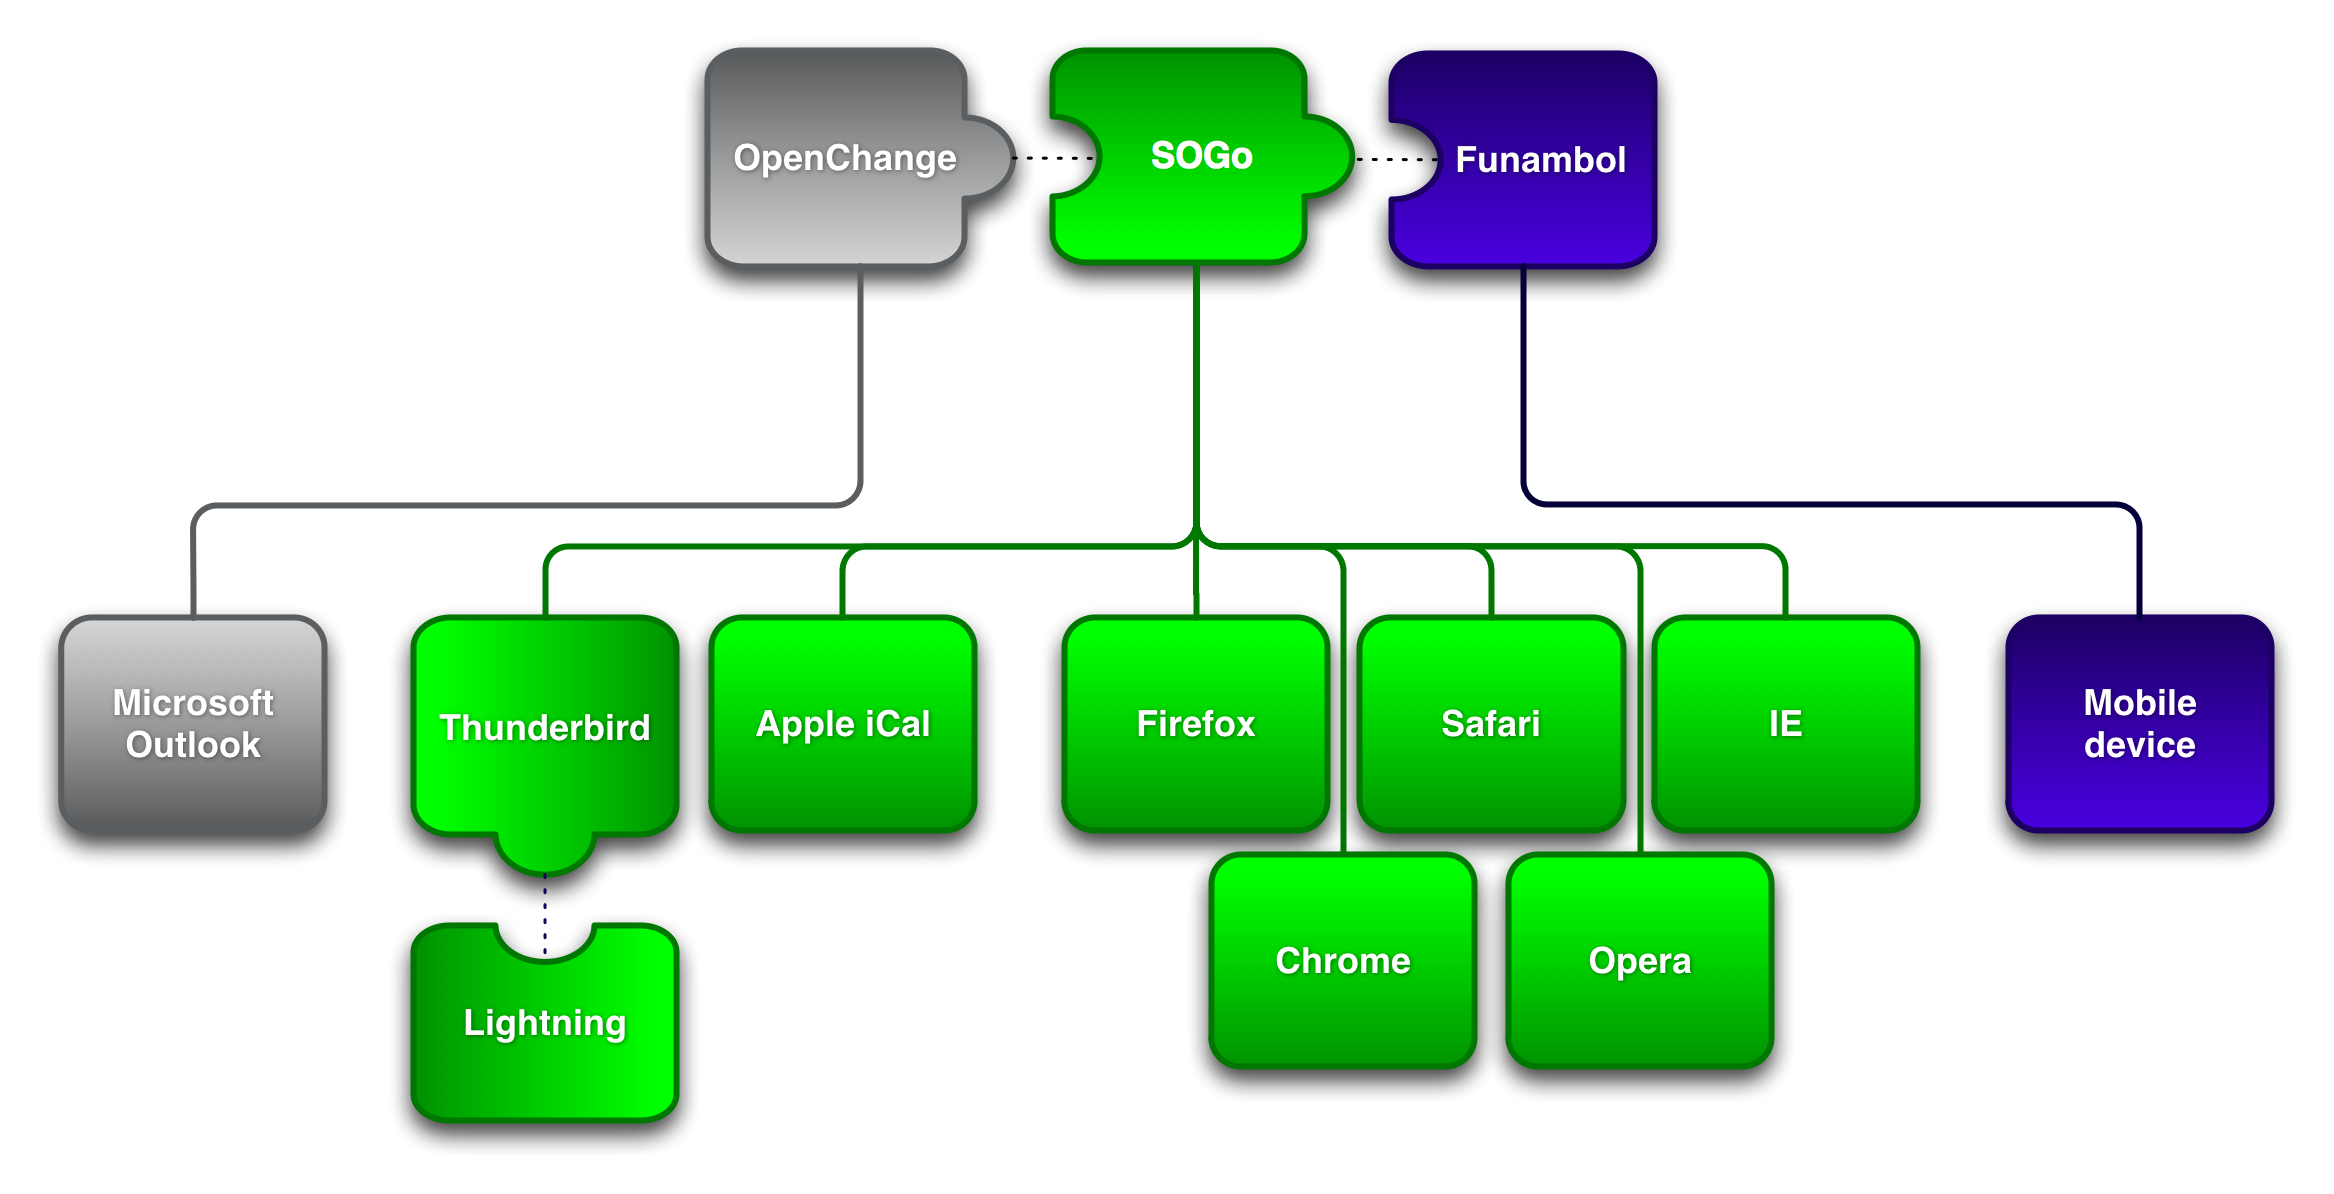
\includegraphics{architecture.png}

Standard protocols such as CalDAV, CardDAV, GroupDAV, HTTP, IMAP and
SMTP are used to communicate with the SOGo platform or its
sub-components. Mobile devices supporting the SyncML standard use the
Funambol middleware to synchronize information.

To install and configure the native Microsoft Outlook compatibility
layer, please refer to the SOGo Native Microsoft Outlook Configuration
Guide.

\section{System Requirements}

\subsection{Assumptions}

SOGo reuses many components in an infrastructure. Thus, it requires the
following:

\begin{itemize}
\itemsep1pt\parskip0pt\parsep0pt
\item
  Database server (MySQL, PostgreSQL or Oracle)
\item
  LDAP server (OpenLDAP, Novell eDirectory, Microsoft Active Directory
  and others)
\item
  SMTP server (Postfix, Sendmail and others)
\item
  IMAP server (Courier, Cyrus IMAP Server, Dovecot and others)
\end{itemize}

In this guide, we assume that all those components are running on the
same server (i.e., \texttt{localhost} or \texttt{127.0.0.1}) that SOGo
will be installed on. Good understanding of those underlying components
and GNU/Linux is required to install SOGo. If you miss some of those
required components, please refer to the appropriate documentation and
proceed with the installation and configuration of these requirements
before continuing with this guide.

\subsection{Software recommendations: More recent versions of the
software mentioned above can also be used.}

\begin{longtable}[c]{@{}ll@{}}
\hline\noalign{\medskip}
\begin{minipage}[t]{0.22\columnwidth}\raggedright
Database server
\end{minipage} & \begin{minipage}[t]{0.46\columnwidth}\raggedright
PostgreSQL 7.4 or later
\end{minipage}
\\\noalign{\medskip}
\begin{minipage}[t]{0.22\columnwidth}\raggedright
LDAP server
\end{minipage} & \begin{minipage}[t]{0.46\columnwidth}\raggedright
OpenLDAP 2.3.x or later
\end{minipage}
\\\noalign{\medskip}
\begin{minipage}[t]{0.22\columnwidth}\raggedright
SMTP server
\end{minipage} & \begin{minipage}[t]{0.46\columnwidth}\raggedright
Postfix 2.x
\end{minipage}
\\\noalign{\medskip}
\begin{minipage}[t]{0.22\columnwidth}\raggedright
IMAP server
\end{minipage} & \begin{minipage}[t]{0.46\columnwidth}\raggedright
Cyrus IMAP Server 2.3.x or later\\Dovecot 2.x or later
\end{minipage}
\\\noalign{\medskip}
\hline
\end{longtable}

\subsection{Minimum hardware requirements:}

\begin{longtable}[c]{@{}ll@{}}
\hline\noalign{\medskip}
\begin{minipage}[t]{0.19\columnwidth}\raggedright
Server
\end{minipage} & \begin{minipage}[t]{0.81\columnwidth}\raggedright
Evaluation and testing\\- Intel, AMD, or PowerPC CPU 1 GHz\\- 512 MB of
RAM (without Funambol, 1 GB RAM otherwise)\\- 1 GB of disk space\\
\end{minipage}
\\\noalign{\medskip}
\begin{minipage}[t]{0.19\columnwidth}\raggedright
\end{minipage} & \begin{minipage}[t]{0.81\columnwidth}\raggedright
Production\\Intel, AMD or PowerPC CPU 3 GHz\\2048 MB of RAM\\10 GB of
disk space (excluding the mail store)\\
\end{minipage}
\\\noalign{\medskip}
\begin{minipage}[t]{0.19\columnwidth}\raggedright
Desktop
\end{minipage} & \begin{minipage}[t]{0.81\columnwidth}\raggedright
Intel, AMD, or PowerPC CPU 1.5 GHz 1024x768 monitor resolution 512 MB of
RAM 128 Kbps or higher network connection
\end{minipage}
\\\noalign{\medskip}
\begin{minipage}[t]{0.19\columnwidth}\raggedright
\end{minipage} & \begin{minipage}[t]{0.81\columnwidth}\raggedright
Microsoft Windows Microsoft Windows XP SP2 or later versions
\end{minipage}
\\\noalign{\medskip}
\begin{minipage}[t]{0.19\columnwidth}\raggedright
\end{minipage} & \begin{minipage}[t]{0.81\columnwidth}\raggedright
Apple Mac OS X Apple Mac OS X 10.2 or later
\end{minipage}
\\\noalign{\medskip}
\begin{minipage}[t]{0.19\columnwidth}\raggedright
\end{minipage} & \begin{minipage}[t]{0.81\columnwidth}\raggedright
Linux Your favourite GNU/Linux distribution
\end{minipage}
\\\noalign{\medskip}
\begin{minipage}[t]{0.19\columnwidth}\raggedright
Mobile devices
\end{minipage} & \begin{minipage}[t]{0.81\columnwidth}\raggedright
Any device supporting the CalDAV and CardDAV standards Apple iPhone /
iPod / iPad using Apple iOS 3.0 or later
\end{minipage}
\\\noalign{\medskip}
\hline
\end{longtable}

\end{document}
